\begin{figure*}[hbt]
\centering
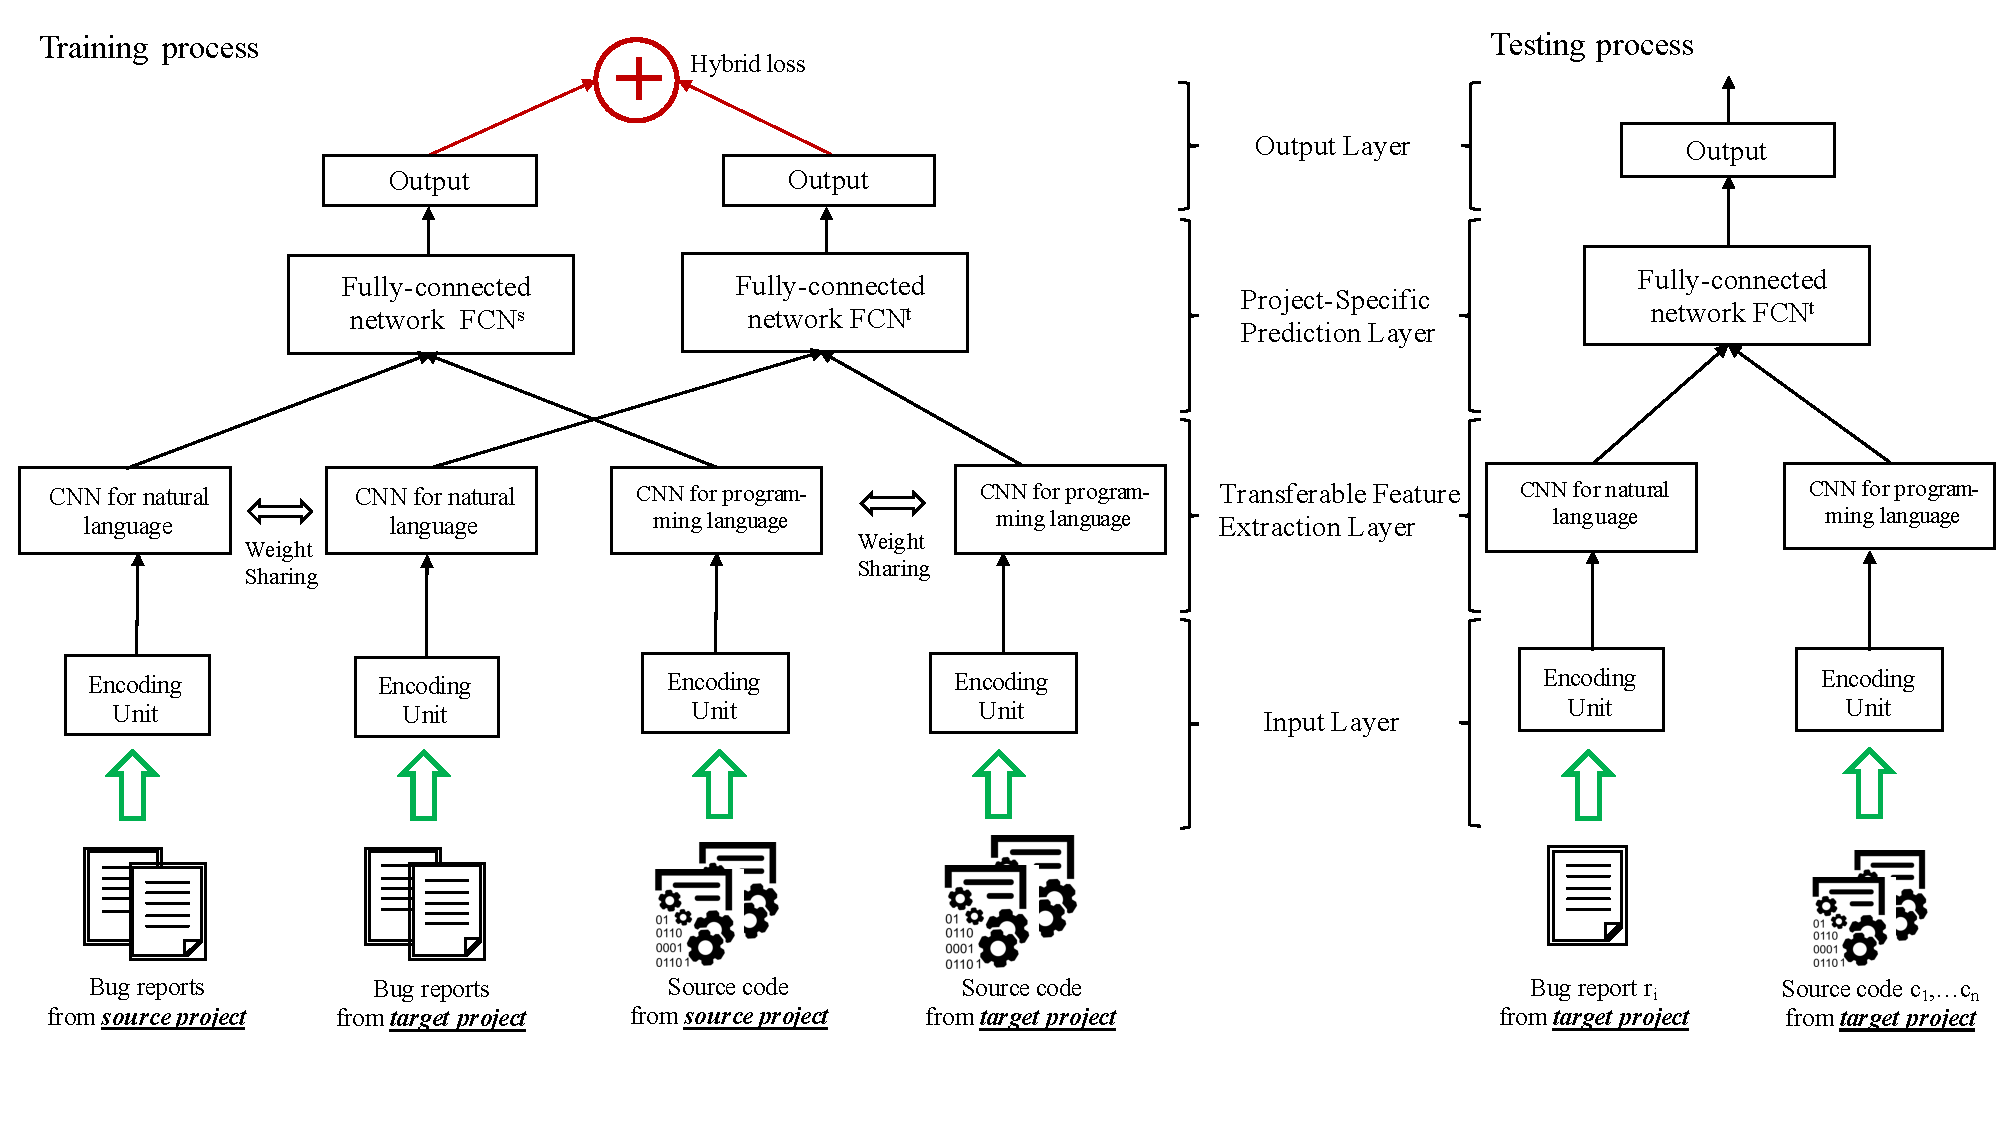
\includegraphics[width = 2\columnwidth]{pic/structure.pdf}
\caption{The overall structure of Transfer Natural and Programming language CNN.  The left part is the training process of \TRANPCNN based on the bug reports and source code from source projects and a few data from target projects, the weights of which are trained by minimizing the loss of ensemble loss from fully-connected networks $fc_s$ and $fc_t$. The right part is the testing process, a new bug report and its candidate source code are fed into the model, and \TRANPCNN outputs their relevant scores for bug localization.}
\label{fig:structure}
\end{figure*}

The goal of cross-project bug localization is using data from source project and a few data from target project to locate the potentially buggy source code in the target project that produce the program behaviors specified in a
given bug report. Let $\mathcal{C}_s =\{ c_{s_1}, c_{s_2}, \cdots, c_{s_{nc_1}}\}$ and $\mathcal{C}_t =\{ c_{t_1}, c_{t_2}, \cdots, c_{t_{nc_2}}\}$ denote the set of source code from source project and target project respectively, $\mathcal{C}=\mathcal{C}_s \bigcup \mathcal{C}_t $. $\mathcal{R}_s =\{ r_{s_1}, r_{s_2}, \cdots, r_{s_{nr_1}}\}$ and $\mathcal{R}_t =\{ r_{t_1}, r_{t_2}, \cdots, r_{t_{nr_1}}\}$ denotes the bug reports, respectively, $\mathcal{R}=\mathcal{R}_s \bigcup \mathcal{R}_t $, where $nc_1, nc_2, nr_1, nr_2$ denote the number of source files and bug reports from source project and target project, respectively. We formulate cross-project bug localization as a learning task which aims to learn a prediction function $f: \mathcal{R} \times \mathcal{C} \mapsto \mathcal{Y}$. $y_{ij} \in \mathcal{Y} = \{+1, -1 \}$ indicates whether a source code $c_j \in \mathcal{C} $ is relevant to a bug report $r_i \in \mathcal{R}$.

In this paper, we propose a novel deep transfer neural network named \TRANPCNN (TRAnsfer Natural and Programm Language Convolutional Neural Network) to instantiate the cross-project bug localization problem, which is an extension of NP-CNN proposed by Huo et al. \TRANPCNN takes the raw data of bug reports and source code as inputs and learns a unified feature mapping $\phi(\cdot, \cdot)$ for a given $r_i$ and $c_j$, based on which the prediction can be made with a subsequent output layer. We will introduce the general framework of \TRANPCNN and explain the way to employ deep transfer technique for cross-project bug localization in the following subsections.

\subsection{General Structure}
The general structure of \TRANPCNN is shown in Figure~\ref{fig:structure}. Specifically, \TRANPCNN consists of four parts: input layer, transferable feature extraction layers, heterogeneous predicting adaptation layers and output layer. The left figure indicates the training process of \TRANPCNN and the right figure indicates the test process. Since the \TRANPCNN model is used to deal with cross-project bug localization tasks, during the training process, pairs of source code and bug reports and ground truth labels from source project are fed into the deep neural network for weight training, as well as very few data from target project, and for testing process, a new bug report from target project and its candidate source code are fed into the model, which outputs their relevant scores indicating which code have high relevance to the given bug report and are located as buggy.



\subsection{Transferable Feature Extraction Layers}
Before processing in Transferable Feature Extraction Layers, the source code and bug reports should be firstly encoded as feature vectors. Traditional techniques usually employs TFIDF to represent text content, which may lose the word relationships. In our model, to maintain the semantics with structural information of text, we apply word2vec technique to encode bug reports and source code.

To process the bug reports in natural language, we follow the standard convolutional neural network~\cite{kim2014convolutional} (named as NCNN) to extract semantic features $\mathbf{h}^r$ from bug reports, which has been widely studied. Meanwhile, as mentioned in Huo et al.~\cite{huo2016learning}, bug reports and source code should be processed in different ways, because two languages have different structural semantic property. Therefore, we apply programming language specific convolutional neural network (named as PCNN) to extract semantic features from source code. The PCNN is able to preserve the integrity within statements by sliding convolutional windows within statements in the first convolutional and pooling layers, and generates semantic features between statements by applying  different sizes of convolutional windows in the subsequent convolutional and pooling layers. The details of PCNN is introduced in the background section and more details can be referred in Huo et al.'s work~\cite{huo2016learning}.

%Source code in programming language, although in textural format, differs from natural language mainly in two aspects. First, the basic language component carrying meaningful semantics in natural language is word or term, and the semantics of the natural language can be inferred from a bag of words. By contrast, in programming language the basic language component carrying meaningful semantics is statement, and the semantics of the programming language can be inferred from the semantics on multiple statements plus the way how these statements interact with each other along the execution path. Thus, to extract features from programming language, the convolution operations should explicitly respect to the atomicity of statements in semantics. Second, natural language organizes words in a ``flat'' way while programming language organizes its statements in a ``structured'' way to produce richer semantics. For example, a branching structure ``if-then-else'' defines two parallel groups of statements. Each group interacts with the statements before and after the branching block while there is no interaction between the two groups. Thus, to extract features from programming language, the convolution operations should obey the program structure defined by the programming languages.

Although the data distribution of cross-projects may be different, the semantics within the statements may be similar since the projects are using the same programming language so that the rule of semantic feature extraction is transferable. Therefore, in the training process, the PCNN models in the transferable feature extraction layers for processing source projects data and target projects data share the same parameter weights, which means that the rule to extract semantic features from programming languages are the same. This structure helps generate semantic features from target project using the large number of training source code in the source projects, leading to a better feature representation in the cross-project bug localization. 
 
\subsection{Heterogeneous Predicting Adaptation Layers}
After processing from transferable feature extraction layers, the high-level semantic features from bug reports and source code are extracted, which would be then fed into a fully-connected neural network for feature fusion. However, in cross-project bug localization, the data distribution of source project and target project is different, which means directly employing the same fully-connected network to fuse features from both source and target projects will have bias, leading to a poor bug localization performance.

One question arises here: can we design a particular network to extract features within project, and fuse feature in separate structure? To address this problem, we design two particular fully-connected networks to combine the middle-level features in Cross-project feature fusion layers: One fully-connected network $fc_s$ is used for source project feature fusion and the other fully-connected work $fc_t$ is used to fuse features in the target project. The structure suggests that the feature extraction of different projects are similar and can be processed in the same Convolutional Neural Network, and the feature fusion and projection process is different so that two separate fully-connected neural network are designed to solve this problem. The objective function in the cross-project feature fusion layers can be rewritten in Eq.~(\ref{eq:lossfunction}):
\begin{equation}
\begin{aligned}
\label{eq:lossfunction}
\mathop{\arg\min}_{\mathbf{W}}&\sum_{s_i,s_j}\mathcal{L}(\mathbf{h}_{s_i},\mathbf{h}_{s_j}
,y_{s_{ij}}; W_{fc_s}, W_{conv} ))\\
+&\sum_{t_i,t_j}\mathcal{L}(\mathbf{h}_{t_i},\mathbf{h}_{t_j},y_{t_{ij}}; W_{fc_t}, W_{conv})+\lambda||\mathbf{W}||^2
\end{aligned}
\end{equation}
where, $\mathcal{L}$ is the square loss, $\lambda$ is the trade-off parameter and the weight vectors $W$ contains the weight vectors in convolutional neural networks $W_{conv}$, in fully-connected network of source domain $W_{fc_s}$ and in fully-connected network of target domain $W_{fc_t}$. All the weights is learned by minimizing the objective function based on SGD (stochastic gradient descent) in the same time.


%cross-language feature fusion layers, where a fully-connected network is employed for learning a unified features and followed by an output layer mapping to the predictions $\mathcal{Y}$. However, a reported bug may only relevant to one or a few source code, while a large number of source code are irrelevant and this imbalance nature should be considered. Similar to~\cite{huo2016learning} which introduced an unequal misclassification cost to handle imbalance problem, we randomly drop some negative instances in the cross-language feature fusion layer, which can decrease the computational cost and counteract the negative influence of the imbalance nature. Let $y_{i}^{(k)}$ denote the $k$-th label of instance $\mathbf{x}_i$ and $\tilde{y}_{i}^{(k)}$ denote its prediction, similar to traditional LSTM model, we use cross entropy error function in the output layer, and the parameters are learned by minimizing the following loss function using stochastic gradient descent (SGD) method: 